\documentclass[conference]{IEEEtran}
\IEEEoverridecommandlockouts
% The preceding line is only needed to identify funding in the first footnote. If that is unneeded, please comment it out.
\usepackage{cite}
\usepackage{amsmath,amssymb,amsfonts}
\usepackage{algorithmic}
\usepackage{graphicx}
\usepackage{textcomp}
\usepackage{xcolor}
\graphicspath{ {./figures/} }
\def\BibTeX{{\rm B\kern-.05em{\sc i\kern-.025em b}\kern-.08em
    T\kern-.1667em\lower.7ex\hbox{E}\kern-.125emX}}
    

\begin{document}

\title{Personalized phenotype encoding and prediction of pathological development from cross-sectional images.\\
\thanks{Identify applicable funding agency here. If none, delete this.}
}
%we have more than 3 authors, so we are allowed to use the long format

\author{\IEEEauthorblockN{Connor Elkhill\IEEEauthorrefmark{1}, Ines. A Cruz-Guerrero, PhD\IEEEauthorrefmark{1}, Jiawei Liu, MS\IEEEauthorrefmark{1}, Marius George Linguraru, DPhil\IEEEauthorrefmark{2, 3},\\Allyson Alexander, MD\IEEEauthorrefmark{4}, Brooke French, MD\IEEEauthorrefmark{5}, Antonio R. Porras, PhD \IEEEauthorrefmark{1,6}}
\IEEEauthorblockA{\IEEEauthorrefmark{1}Department of Biostatistics and Informatics, Colorado School of Public Health, Aurora, CO}
\IEEEauthorblockA{\IEEEauthorrefmark{2}Sheikh Zayed Institute for Pediatric Surgical Innovation, Children's National Hospital, Washington, DC}
\IEEEauthorblockA{\IEEEauthorrefmark{3}Departments of Radiology and Pediatrics,George Washington University\\School of Medicine and Health Sciences, Washington, DC}
\IEEEauthorblockA{\IEEEauthorrefmark{4}Department of Pediatric Neurosurgery, Children's Hospital Colorado, Aurora, CO}
\IEEEauthorblockA{\IEEEauthorrefmark{5}Department of Pediatric Plastic and Reconstructive Surgery, Children's Hospital Colorado, Aurora, CO}
\IEEEauthorblockA{\IEEEauthorrefmark{6}Departments of Pediatrics, Surgery and Biomedical Informatics, School of Medicine, Aurora, CO\\Email: connor.2.elkhill@cuanschutz.edu}
}


\maketitle

\begin{abstract}
The prediction of anatomical development plays a crucial role in pediatric treatment selection and planning. We present a novel deep learning architecture to make personalized predictions of pediatric normative and pathologic head development using only cross-sectional data. We designed growth predictor that learns the anatomical effects of age and sex in the presence of pathology and a novel phenotype encoder that utilizes domain adversarial training to create age- and sex-independent representations of patient phenotypes. We combined these modules to instantiate patient phenotypes to specific ages for personalized anatomical predictions conditioned to cranial pathology. We trained our models using standardized head segmentations generated from cross-sectional CT images and 3D photograms and evaluated model performance using an independent longitudinal dataset of normative subjects and children with craniosynostosis. The model achieved a head surface growth prediction error of 4.93 ± 2.29 mm and a volumetric error 0.17 ± 0.11 L in patients with cranial pathology, and 4.61 ± 3.28 mm and 0.27 ± 0.19 L for normative subjects, demonstrating state-of-the-art accuracy. Our method is the first to create age- and sex-agnostic phenotypical representations and enable personalized predictions of pathological development from only cross-sectional data.
\end{abstract}

\begin{IEEEkeywords}
predictive growth, craniosynostosis, generative adversarial network, domain adversarial training, pediatric pathological development
\end{IEEEkeywords}

\section{Introduction}
Children undergo a rapid cranial and brain growth during the first few years of life that is crucial for their cognitive development \cite{Cao2017Developmental}. Craniosynostosis is a condition where one or more of the cranial sutures fuse prematurely and constrain cranial and brain development, often requiring surgical intervention~\cite{Mathijssen2021Updated}. However, current clinical standards to evaluate developmental anomalies rely on normative growth charts of simple metrics such as head circumference, cephalic index, or intracranial volume~\cite{Likus2014Cephalic, Meyer-Marcotty2014Three-dimensional, Rollins2010United} that cannot characterize or predict development of patients with pathology ~\cite{Breakey2018Intracranial, Sgouros2005Skull, Thakkar2018Observer}.

Several methods to predict cranial growth without longitudinal training datasets have recently been proposed. Liu et al~\cite{Liu2022Data-driven} created a normative reference of cranial growth based on age and sex using principal component analysis and temporal regression. However, this method is not personalized and only identified average growth trajectories in the normative pediatric population. Porras et al~\cite{Porras2022Predictive} presented a personalized predictive model of cranial growth, but the optimization was not computationally feasible for large datasets. Recently, Liu et al~\cite{Liu2023Data-driven} presented a data-driven model of cranial suture growth trained only with cross-sectional data, and demonstrated state-of-the-art accuracy to predict pathologic development in patients with craniosynostosis. However, this method required the observation of the cranial sutures from computed tomography (CT) images, an image modality that requires harmful radiation exposure~\cite{Schweitzer2012Avoiding}. In a different domain, Xia et al~\cite{Xia2021Learning} utilized generative adversarial networks to learn subject-specific trajectories from a cross-sectional dataset of magnetic resonance (MR) images to predict changes in the brain morphology of patients with Alzheimer’s disease. However, their paired training scheme prevented significant anatomical temporal changes, which provided good results in adults but is not realistic in children~\cite{Hasegawa2018Developmental}.

As an alternative to CT imaging, 3D photogrammetry has become a popular radiation-free and low-cost clinical alternative to evaluate pediatric cranial malformations~\cite{Porras2019Quantification, Abdel-Alim2021Three-Dimensional}. However, it can only image the head surface and hence, prior personalized  methods~\cite{Liu2023Data-driven} relying on the identification of the cranial sutures are not feasible. We present a novel deep learning architecture designed to make personalized predictions of normative and pathologic development trained using head surface information from both cross-sectional CT images and 3D photograms, which enables radiation-free prediction of pediatric development in a clinical setting. We propose a temporal growth predictor based on a conditional generative adversarial network that learns age- and sex -specific anatomical distributions with or without the presence of pathology in the pediatric population. We also present a novel phenotype encoder that utilizes domain adversarial training, avoiding the stringent statistical assumptions of prior works, to generate age- and sex-agnostic latent representations of patient phenotypes. These modules work collaboratively to generate personalized predictions of anatomical development by instantiating patient-specific phenotype representations to specific ages conditioned to the presence of pathology. The architecture was trained using only cross-sectional data from normative children and patients with craniosynostosis under the age of 10 years and was evaluated using an independent longitudinal dataset.
\section{Materials and Methods}
\subsection{Data}
After IRB approval at XXXXXXXXXXXXXXXXX (\#XXXXXXXXXXXXXXXX) we collected two independent retrospective datasets: (1) a cross-sectional dataset used for model training; and (2) a longitudinal dataset used for performance evaluation. \textbf{Dataset 1} includes 2,672 cross-sectional CT images (N=2,262) and 3D photograms (N=410) of two patient populations: 2,020 normative subjects without cranial pathology (1081 male, 939 female, age $3.14 \pm 3.05$ years, range 0-10 years) and 652 patients with craniosynostosis (384 male, 268 female, age $0.64 \pm 1.04$ years, range 0-8.8 years). Dataset 2 includes two groups of longitudinal images: 61 CT image pairs from 51 normative subjects (28 male, 23 female) with average age at first image $2.24 \pm 2.22$ years and age at second image $3.55 \pm 2.71$ years (five subjects had two image pairs); and 75 pairs of 3D photograms from 75 patients with craniosynostosis (58 male, 17 female), with age of $0.61 \pm 1.07$ years at the first image and $0.85 \pm 1.18$ years at the second image.
\begin{figure}[!b]
\centering
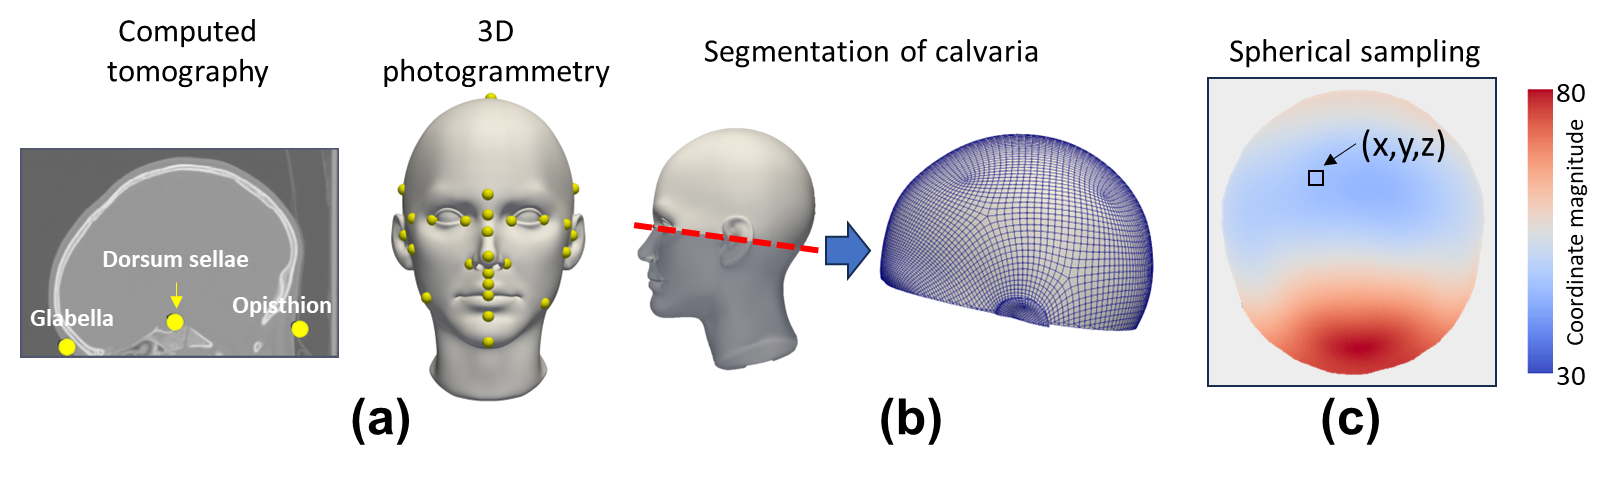
\includegraphics[width=\columnwidth]{figures/StandardizedRepresentation.png}
\caption{Standard representation of the head surface. (a) CT image or 3D photogram annotated with anatomical landmarks. Detailed annotations of landmarks for 3D photograms can be found in~\cite{Elkhill2023Geometric}. (b) Segmented head surface using the naso-tragal plane. (c) Two-dimensional standard representation of the head surface using spherical sampling, where each pixel contains the corresponding location in the head surface (X, Y, Z).}
\label{fig:standard}
\end{figure}
\subsection{Standard representation of the head surface}
We used publicly available methods to segment the head surface from CT images and 3D photograms and create standardized 2D anatomical representations~\cite{Porras2022Predictive}. In summary, adaptive thresholding~\cite{Liu2022Data-driven} and the marching cubes algorithm~\cite{Lorensen1987Marching} were used to segment the head surface from a CT image. Four cranial landmarks were automatically identified at the glabella, two temporal processes of the dorsum sellae and the opisthion in CT images. In 3D photogrammetry, we used a similar publicly available method to identify a series of anatomical landmarks on the head and face~\cite{Elkhill2023Geometric}. We used a standardized template image annotated with both sets of landmarks to align the images from both modalities given their respective landmarks. We segmented the calvaria from the rest of the head at the cranial base using the plane defined by the nasion, left and right tragion annotated on the standardized template (Fig \ref{fig:standard}b). Finally, the head surface segmented from either image modality was sampled in spherical coordinates to create a standard 2D representation~\cite{Porras2022Predictive} Fig \ref{fig:standard}c.
\subsection{Model architecture}
We propose a neural network architecture composed of two main modules as presented in \ref{fig:architecture} and described below.
Personalized phenotype encoder (PPE). The goal of this module is to create a vectorized representation of the head phenotype of a patient independently from age and sex. To accomplish this, we designed a phenotype encoder that uses unsupervised representation learning and the convolutional architecture presented in~\cite{Radford2016Unsupervised} to provide a latent patient-specific phenotype representation l based on a real head shape observation \textbf{X}. Unlike previous work, we incorporate an additional phenotype discriminator (PD, purple in \ref{fig:architecture}) and use a domain adversarial training scheme~\cite{Ganin2016Domain-Adversarial} (see details in section 2.4, Eq. 1)%todo-ref here
to promote a phenotype representation l that is independent from age or sex. Hence, the encoder will learn to generate latent phenotype representations l that cannot be used by the PD to identify the age and sex of the patient.
Growth predictor (GP). This module uses an adversarial training scheme with the goal of generating a realistic head surface anatomy from a latent representation of a head phenotype \textbf{l} (generated by the PPE) together with information about age, sex and pathology by leveraging the learned anatomical distributions of specific patient groups in the training dataset. The GP and PPE work collaboratively to create personalized latent phenotype representations that are age- and sex-agnostic and that, when combined with specific age, sex, and pathology information, can represent the head anatomy of a specific patient. The predictor follows the convolutional architecture proposed by~\cite{Radford2016Unsupervised} but it was modified to include the conditions of patient age (encoded as a continuous variable), sex (binary encoded) and suture fusion status (one-hot encoded).
Finally, the growth discriminator (GD) (Fig \ref{fig:architecture}, in green) enables adversarial training of both the GP and PPE. The discriminator also utilizes the convolutional architecture proposed in~\cite{Radford2016Unsupervised} to compute the Wasserstein distance~\cite{Gulrajani2017Improved} and distinguish between real head shapes and head shapes reconstructed from \textbf{l}.
\subsection{Optimization}
We defined the prediction of age and sex from the PD as $S',A'=PD(l;\theta_{PD})$ respectively, where $\theta_{PD}$ are the learned parameters of the PD and \textbf{l} is the latent representation generated from the PPE using real input image \textbf{X}. Similar to~\cite{Wang2021Deep}, we computed the cross entropy between $S$ and $S'$ and KL divergence between the continuous distributions of $A$ and $A'$, where $A$ and $S$ are the true patient age and sex. The PPE and PD modules are trained using the following adversarial loss function:
\begin{equation}
    \begin{split}
    L_{PPE}=\underset{PPE}{max}\ \underset{PD}{min}\ S*log(S')\\+(1-S)*log(1-S')+ A *log\frac{A}{A'}
    \end{split}
\end{equation}
To train the GP module, we used an adversarial scheme with the following Wasserstein loss function~\cite{Gulrajani2017Improved}.
\begin{equation}
    \begin{split}
    L_{GP}=E_{{X^-~P_l}|X_{P_x}}
    \end{split}
\end{equation}

\begin{figure}[!t]
\centering
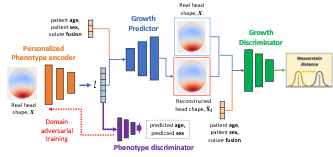
\includegraphics[width=\columnwidth]{figures/NetworkArchitecture.png}
%todo -- replace this with an SVG
\caption{Proposed neural network architecture. The personalized phenotype encoder creates a latent representation of a patient phenotype l from a real head shape that is independent of patient age or sex using domain-adversarial training. The growth predictor is trained to predict head anatomies consistent with the observed statistical distributions in the population for specific age, sex, and suture fusion status. Once trained, the phenotype representation of a patient l can be instantiated at any age using the growth predictor to produce personalized predictions.}
\label{fig:architecture}
\end{figure}
\bibliographystyle{ieeetr}
\bibliography{ref-extracts}
\end{document}
